\documentclass[12pt,a4paper]{article}
\usepackage[margin=1in]{geometry}
\usepackage{tikz}
\usetikzlibrary{arrows.meta}
\usepackage[T1]{fontenc}
\usepackage[utf8]{inputenc}
\usepackage{mathptmx,microtype,booktabs,longtable,array,xcolor,enumitem,parskip}
\usepackage[hidelinks]{hyperref}
\setlength{\emergencystretch}{3em}
\setlist{nosep}
\newcolumntype{P}[1]{>{\raggedright\arraybackslash}p{#1}}
\newcommand{\red}[1]{\textcolor{red}{#1}}
\title{GPU Sharing Mechanisms for Multi-Tenant Inference Serving:\\An Evidence-Based Operating Systems Engineering Review}
\author{Muhammad Burhan Un Nadeem (SE-24071)\\Muhammad Faaiz Alam (SE-24094)\\Ali Raza (SE-24302)}
\date{Group A --- Operating Systems Complex Engineering Problem\\NED University of Engineering and Technology\\17 October 2026}
\begin{document}
\maketitle
\begin{abstract}
Sharing an accelerator among inference tenants can improve useful capacity, yet contention changes latency and the meaning of isolation depends on the mechanism. We review temporal scheduling, NVIDIA Multi-Process Service (MPS), Multi-Instance GPU (MIG), and API-level remoting or virtualization with single-device inference evidence as the technical unit. A submitted protocol guides four publisher-platform searches and source-anchored screening. \red{The current 43 accepted primary studies are a working set, not a completed final systematic selection: 45 extension reports await assessment, 96 earlier reports have unresolved retrieval, and four record links await adjudication.} We distinguish same-experiment effects from cross-paper interpretation, and separate throughput, SLO goodput, latency percentiles, resource separation, security and fault containment. The evidence supports conditional choices: temporal control for strict priority when its scheduling constraints fit; tuned MPS for packing compatible inference; MIG for explicit partitioning where hardware, profiles and memory fit; and API control when interception and data movement fit the latency budget. Hybrids require local validation. \red{These recommendations must be checked against the completed selection and missing configuration fields before submission.}
\end{abstract}
\noindent\textbf{Status and marking convention.} Red text denotes an open decision, a provisional count, or an interpretation to revisit. Black study observations are bounded to the cited source and its extracted experiment; they do not make the review final. The companion \texttt{cep\_report.txt} retains red passages as \texttt{[RED: ...]} markers. This manuscript is a substantive CEP draft for review, not a claim that the unresolved PRISMA flow is complete.
\newpage\tableofcontents\newpage

\section{Introduction}
In a multi-tenant inference server, requests from distinct models or clients compete for execution slots, accelerator memory, caches and memory bandwidth. Exclusive GPU allocation simplifies attribution of latency to a tenant but can leave capacity idle when individual jobs are small or bursty. Concurrent execution can raise aggregate useful work while delaying a high-priority request, especially when the co-tenant's kernel or transfer pattern is unpredictable. Selecting a sharing mechanism is therefore an operating-systems decision about admission, scheduling, resource boundaries and observability, rather than a single throughput benchmark.

The assigned alternatives operate at different layers. Time-slicing switches or queues work over time; MPS enables multi-process execution and configurable active-thread shares; MIG presents hardware-defined GPU instances on supported NVIDIA devices; API remoting or virtualization routes calls, context state or data through an additional control path. Research systems frequently combine these with batching, model placement, kernel interception, memory management and feedback control. Such combinations cannot be evaluated as if one toggle alone produced the reported gain. The unit of our central comparison is concurrent inference on one physical GPU; multi-GPU outcomes are context unless a local sharing experiment can be identified.

We ask five analytical questions. \textbf{RQ1:} Which sharing/control mechanisms and boundaries have been evaluated for multi-tenant inference? \textbf{RQ2:} Which utilization, density, latency, fairness and isolation outcomes are actually measured, and which are comparable? \textbf{RQ3:} Under what workload, hardware and configuration conditions do results change? \textbf{RQ4:} What trade-offs and contradictory evidence emerge, and what experimental differences may explain them? \textbf{RQ5:} Which choice is defensible under stated requirements and evidence limits? The answers are synthesized in Sections 5--10, rather than determined by counting papers in each category.

\section{Research Questions}
The review answers five questions derived from the assigned comparison. RQ1 asks which temporal, MPS, MIG, API and hybrid controls have direct local inference evaluations. RQ2 asks how density, goodput, latency, fairness and isolation are measured and which comparisons are commensurable. RQ3 asks which hardware, model, concurrency and arrival conditions change results. RQ4 asks which conflicting effects and engineering costs are observed. RQ5 asks what choice is supported for a stated SLO, capacity, hardware and isolation requirement. Each question requires evaluation rather than a list of titles; the evidence requirements and corresponding outputs are detailed in Sections 3--10.
\section{Research Methodology}
\subsection{Protocol, eligibility and review procedure}
The submitted \texttt{SLR\_protocol.tex/pdf} is the baseline. Its Group A execution record and dated amendments are in \path{groups/group-a/protocol.md} and \path{evidence/protocol_amendments.md}. The literature cutoff was extended to 11 October 2026. The study must be an English-language, peer-reviewed original full journal or conference report with relevant concurrent inference evidence and adequate technical detail; mixed inference/training work is used only where the inference result is separately identifiable. Training-only, cluster-only, editorial, survey and vendor-only material does not enter the primary set. A report-version link does not create an additional underlying study. Source retrieval failure remains an access outcome, not an eligibility exclusion.

One AI reviewer carried out the recorded screening and quality appraisal under the user's instruction. This is a limitation, not a claim of independent student consensus. Stable record, report and study IDs, reasons and extraction anchors are retained in the supporting workbook and CSV files. Quality uses ten criteria scored 0, 0.5 or 1, yielding a total out of 10; it assesses reporting and experimental adequacy, not proof of a mechanism's causal superiority. \red{A human audit of screening, quality scoring and the remaining reports is still needed.}

\subsection{Databases, strings and counts}
The NED E.A. Khan Library E-Resources listing motivated IEEE Xplore, Springer Nature Link, ACM Digital Library and ScienceDirect. The exact platform-specific Boolean strings, filters, interface URLs, dates and export filenames are preserved in \texttt{search\_runs.csv} and \texttt{search\_runs\_received.csv}; the executable strings are too long to replace with a falsely standardized shorthand here. The common concept combines GPU with inference/model serving terms and the relevant temporal, MPS, MIG or virtualization family. IEEE used four family searches; Springer and ACM used broader master searches; ScienceDirect used four family searches after the master exceeded the interface connector limit. The ScienceDirect split also dropped DNN/LLM synonyms from the common block, a documented recall limitation. Supplementary discovery is identified separately and Google Scholar is not treated as a formal database.

The 11 October IEEE/Springer capture has 689 formal occurrences (102 IEEE, 587 Springer). The supplied ACM/ScienceDirect exports have 3,727 parsed occurrences (1,829 ACM, 1,898 ScienceDirect), for \red{4,416 parsed formal occurrences across the four sources}. ACM displayed 1,600 or 1,603 hits in different saved observations while exports contain 1,829 rows; ScienceDirect MPS displayed 517 in an earlier note and 563 upon later reopening. These differences are preserved rather than silently normalized. A displayed hit count, parsed export row and unique report have different denominators. No publisher entitlement or complete coverage is inferred from an E-Resources listing.

\subsection{Evidence units and study selection}
The protocol uses three linked identities. An occurrence is one result as exported or captured from a run; a report is a specific full publication, including a later journal version; and a study is the distinct underlying evaluation. This distinction prevents counting a paper found in several databases more than once or treating a conference paper and its journal extension as independent experiments. DOI and title matching propose duplicate links, but ambiguous versions require a recorded decision. For example, the journal REEF report is preferred for GA-S001 and its earlier conference report remains linked history \cite{reef}. A different title or DOI is not sufficient by itself to prove a separate evaluation.

Title and abstract decisions use the protocol's scope criteria, with uncertainty advanced rather than forced into an exclusion. Retrieval attempts are recorded separately; inability to obtain a full text cannot be presented as an assessment of its evidence. At full text the reviewer applies one principal reason: E1 no inference-serving evidence; E2 no local multi-tenant sharing; E3 mechanism outside scope; E4 training only; E5 cluster only without separable local data; E6 non-primary or non-peer-reviewed report; E7 insufficient detail; E8 duplicate or less complete report; E9 period or language; E10 a documented other reason. These are decision categories, not an estimate of the unresolved queue's fate. The working set admits mixed training/inference studies only for separable inference outcomes and labels any transferred inference claim as such.

\subsection{Quality assessment and extraction}
All 43 working studies have a Q1--Q10 appraisal row with item scores and rationales. Each item receives 1, 0.5, or 0, with high (8--10), moderate (6--7.5), and low (below 6) reporting bands. Q1 checks the tenant question; Q2 the mechanism; Q3 hardware and software; Q4 workload; Q5 comparator; Q6 metrics; Q7 measurement controls; Q8 support for a result; Q9 limitations; and Q10 interpretability. The item-level matrix and checklist are in Appendix B. The total is a guide to how fully an evaluation can be interpreted; a high-scoring paper can still be indirect for this project's one-GPU decision or omit adversarial tests. No study was made eligible because it had a high score.

The extraction form records identity and report version; source type and access; GPU/SKU/count, OS, driver, runtime, partition/quota; model size and inference task; tenants, co-tenants, batch, arrival and measurement window; comparator; statistic and unit; bounded result; caveat; and page, figure or table anchor. Source-derived observation and reviewer inference are kept apart. The published CSV has separate performance interference, resource/memory, security, and fault-containment fields. A blank chart coordinate or unspecified driver is marked untranscribed where appropriate, rather than supplied from product defaults. The Appendix C cards reproduce a single bounded outcome and caveat per preferred report; the full workbook remains the evidence record for individual results.

\subsection{Synthesis plan and sensitivity}
The protocol calls for a structured narrative synthesis because workloads, accelerators, control layers, latency percentiles and resource budgets differ. Within-study matched comparisons can support a bounded direction or numeric effect in that paper's stratum. Across studies we compare conditions and mechanisms qualitatively; we do not average heterogeneous ratios or equate a server's GPU count to local occupancy. Findings are classified as direct within-study evidence, indirect transfer to the assigned decision, contextual mechanism description, or insufficient evidence. RQ1 uses the control-boundary taxonomy; RQ2 the metric and comparator audit; RQ3 the hardware/workload strata; RQ4 adverse examples and competing objectives; RQ5 a conditional decision table. A final sensitivity analysis must revisit recommendations after excluding moderate-score or weakly anchored evidence and after resolving the current access queue. \red{The working set has not passed that final sensitivity gate.}

\subsection{Search provenance and deviations}
The IEEE and Springer runs on 11 October and the later ACM and ScienceDirect exports on 14 October are separate events; an earlier blocked pilot is not a successful search. The exact run expressions, fields, filters, date, display observations and source links are rendered in Appendix A and kept in the two search-run CSVs. Springer and ACM use a broad master expression, while IEEE and ScienceDirect use family-specific expressions. The IEEE public search covered all metadata rather than the planned field-qualified command form. ScienceDirect split the master to satisfy its connector limit and omitted DNN/LLM in its shared inference block; this changes recall. ACM's displayed hit total and parsed exports diverge. The ScienceDirect temporal URL indicates an open-access facet whose use at the time of export is not established. These issues cannot be repaired by renaming imported rows. \red{A documented re-export or a formal coverage-limitation decision remains necessary.}

\section{PRISMA 2020 Study Selection}
\subsection{Selection status and provisional stage map}
Figure 1 is an \red{interim stage map}, with arithmetic cross-checked against \path{interim_four_source_prisma.json}. It is deliberately labelled as provisional: four additional links, row-level Step 3--5 decisions, report versions and retrieval statuses still need canonical reconciliation. The 11 October 21-study flow is a separate historical snapshot, and batch additions must not be pasted into its boxes. The 43-study current set combines 21 historical accepted studies with 10, 3 and 9 accepted in three assessed batches. Two earlier eligible reports remain pending formal integration. The queue contains 45 unassessed reports, and 96 older reports remain unresolved for retrieval. \red{The final PRISMA 2020 diagram and final unique-study count cannot yet be certified.}


\begin{figure}[p]
\centering
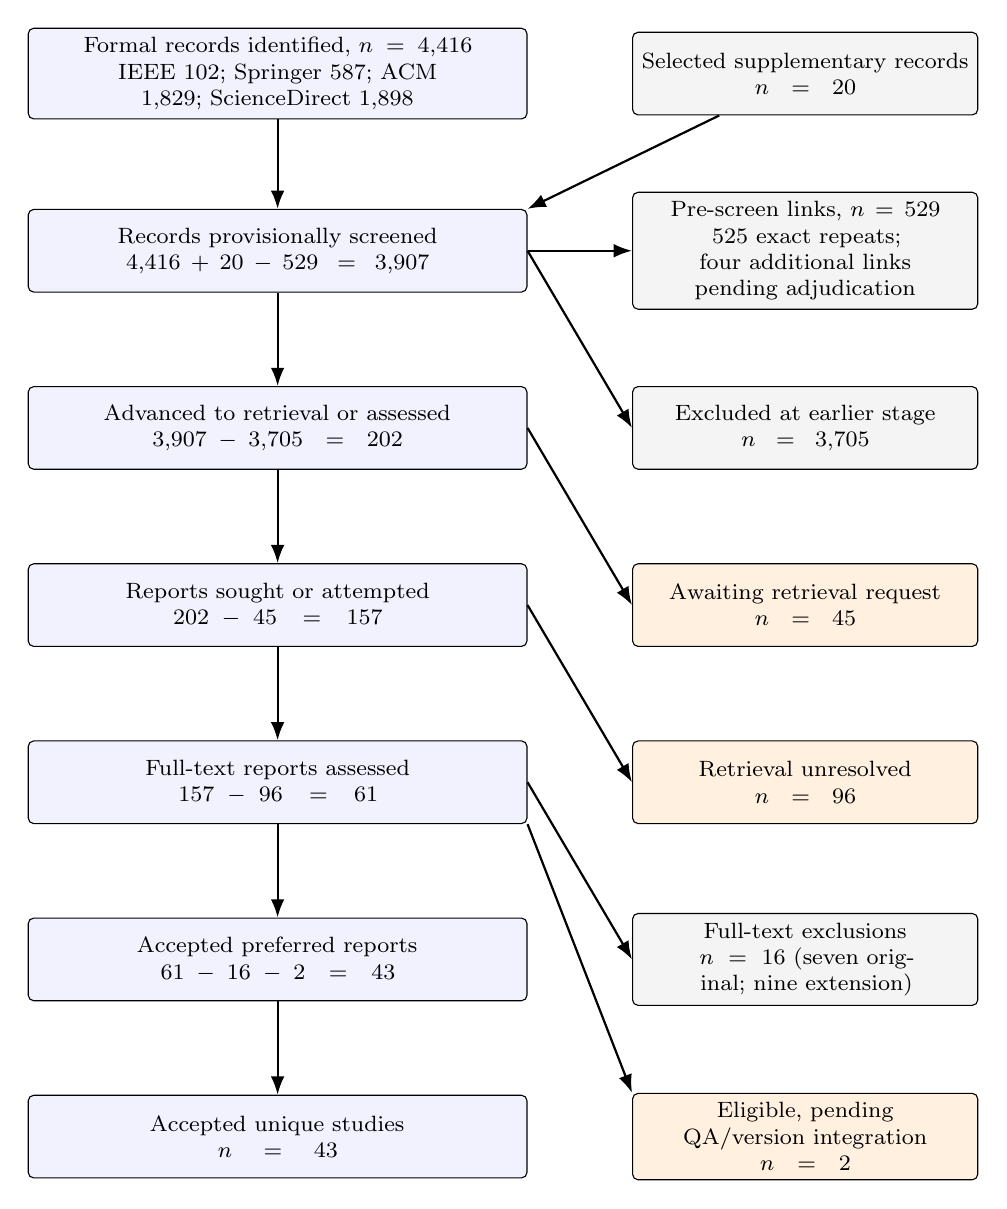
\begin{tikzpicture}[>=Latex, every node/.style={font=\footnotesize},
  main/.style={draw,rounded corners=2pt,align=center,text width=6.1cm,minimum height=1.05cm,fill=blue!5},
  side/.style={draw,rounded corners=2pt,align=center,text width=4.15cm,minimum height=1.05cm,fill=gray!9},
  open/.style={draw,rounded corners=2pt,align=center,text width=4.15cm,minimum height=1.05cm,fill=orange!12},
  line/.style={-Latex,thick}]
\node[main] (identified) at (0,0) {Formal records identified, $n=4{,}416$\\IEEE 102; Springer 587; ACM 1,829; ScienceDirect 1,898};
\node[side] (supp) at (6.7,0) {Selected supplementary records\\$n=20$};
\node[main] (screened) at (0,-2.25) {Records provisionally screened\\$4{,}416+20-529=3{,}907$};
\node[side] (dups) at (6.7,-2.25) {Pre-screen links, $n=529$\\525 exact repeats; four additional links pending adjudication};
\node[main] (advanced) at (0,-4.5) {Advanced to retrieval or assessed\\$3{,}907-3{,}705=202$};
\node[side] (early) at (6.7,-4.5) {Excluded at earlier stage\\$n=3{,}705$};
\node[main] (sought) at (0,-6.75) {Reports sought or attempted\\$202-45=157$};
\node[open] (unsought) at (6.7,-6.75) {Awaiting retrieval request\\$n=45$};
\node[main] (assessed) at (0,-9) {Full-text reports assessed\\$157-96=61$};
\node[open] (unavailable) at (6.7,-9) {Retrieval unresolved\\$n=96$};
\node[main] (accepted) at (0,-11.25) {Accepted preferred reports\\$61-16-2=43$};
\node[side] (excluded) at (6.7,-11.25) {Full-text exclusions\\$n=16$ (seven original; nine extension)};
\node[main] (studies) at (0,-13.5) {Accepted unique studies\\$n=43$};
\node[open] (integration) at (6.7,-13.5) {Eligible, pending QA/version integration\\$n=2$};
\draw[line] (identified) -- (screened);
\draw[line] (supp) -- (screened.north east);
\draw[line] (screened.east) -- (dups.west);
\draw[line] (screened) -- (advanced);
\draw[line] (screened.east) -- (early.west);
\draw[line] (advanced) -- (sought);
\draw[line] (advanced.east) -- (unsought.west);
\draw[line] (sought) -- (assessed);
\draw[line] (sought.east) -- (unavailable.west);
\draw[line] (assessed) -- (accepted);
\draw[line] (assessed.east) -- (excluded.west);
\draw[line] (assessed.south east) -- (integration.north west);
\draw[line] (accepted) -- (studies);
\end{tikzpicture}
\caption{Interim PRISMA 2020 stage map for the four captured database sources and selected supplementary records, 17 October 2026. The 529 pre-screen links include four Step 5 links awaiting canonical record/report adjudication; the 3,907 screening count is provisional. The 45 unsought reports and 96 unresolved retrieval cases are open, and two eligible reports await formal QA and version integration. Counts represent parsed occurrences, not verified search coverage; publisher hit/export discrepancies remain open. Source arithmetic and limitations: \texttt{interim\_four\_source\_prisma.json}.}
\label{fig:prisma-interim-four-source}
\end{figure}
\clearpage

The identities are 4,416+20-525-4=3,907; 3,705+202=3,907; 45+157=202; 96+61=157; and 16+2+43=61. These equations demonstrate arithmetic consistency of the interim map, not that each link, screening event or source coverage has been fully audited. The historical 21-study figure remains a separate checkpoint in the query report; this interim map must not be submitted as a final PRISMA flow.

\subsection{Evidence base, extraction and comparability}
The working set contains 43 distinct accepted study IDs, each with a preferred report, a quality row and a bounded extraction row. The bibliography preserves those report keys. The complete study register in Appendix A gives the title, year, mechanism and quality score; Appendix B maps a concise extracted observation and limitation to the source location. The workbook holds fuller version and screening records. Peer-reviewed status of a venue does not validate all figures or indicate that our team reran its experiments. Some source copies are Markdown conversions with interleaved columns or inaccessible plot pixels; untranscribed values are never interpolated.

We distinguish \emph{request throughput} (all processed requests per unit time) from \emph{SLO goodput} (requests meeting a specified deadline), GPU busy time, SM occupancy, instance count, energy and a paper's custom utilization/efficiency ratio. A lower instance count in a fleet experiment is not a directly measured local GPU occupancy gain. Mean latency, p90/p95/p98/p99, time to first token (TTFT), time between tokens (TBT), job completion time (JCT), and violation rates have different meanings. A paper's p99 under one arrival process cannot be numerically pooled with another paper's mean under a different model, GPU or baseline. InferFair's unfairness ratio is also distinct from security isolation. The evidence matrix therefore uses within-study comparisons and explicitly marks indirect cross-study recommendations.

For an interpretable comparison one must know the GPU SKU and memory, driver/runtime, MIG profile or MPS active-thread quota, model and input/output sizes, batching, tenant mix, arrival trace, SLO definition, comparator resource budget, warm-up and measurement windows, and uncertainty estimate. \red{Some of these parameters remain NOT EXTRACTED in individual records, so a formal effect-size meta-analysis is not justified.} Direct security and injected-fault tests are scarce; interference reduction, resource separation, adversarial confidentiality and fault containment are separate properties.

\section{Classification and Taxonomy of Existing Approaches}
\subsection{Temporal admission, switching and priority}
Clockwork schedules predictable GPU work with SLO-aware goodput as a central outcome \cite{clockwork}. PipeSwitch explores pipelined context switches \cite{pipeswitch}. REEF, Sirius, Orion, XSched, Paella, SPLIT, Miriam, SwitchFlow and ElasticRoom use different combinations of preemption, priority, kernel or subgraph control, compilers and feedback \cite{reef,sirius,orion,xsched,paella,split,miriam,switchflow,elasticroom}. These are not interchangeable implementations of a generic time slice: a scheduler that can intercept launches, preempt selected kernels and control memory handover has a different cost and failure mode from exclusive model execution. SwitchFlow's concurrent inference evidence is in its inference-specific experiment; its larger mixed inference/training p95 example is a separate stratum \cite{switchflow}.

Temporal control is attractive when a small high-priority request should interrupt or avoid best-effort interference. It still needs admitted kernels to finish or be preempted in time, enough memory for models and a credible worst-case workload profile. More aggressive interruption can lower throughput of the best-effort tenant. A priority guarantee is a performance property under evaluated arrivals, not an adversarial security boundary. The strength of this inference is direct for the cited within-study experiments and indirect when generalized to a new GPU or model.

\subsection{MPS and software spatial quotas}
MPS enables simultaneous work and configurable active-thread limits; research systems use it to provision GPUlets, adapt quotas, right-size kernels or shape interference \cite{gpulet,gslice,vastpipe,igniter,fastgshare,admix,deinfer}. Bless and DeInfer add scheduling or prediction, so their gains cannot be assigned to MPS alone \cite{bless,deinfer}. A quota may limit some compute contention while cache, memory traffic and process behavior remain shared. VastPipe's A100 pair and separate AMD CU-mask experiments must not be pooled; the latter is not NVIDIA MPS \cite{vastpipe}. DeInfer directly observes remaining latency interference under MPS spatial allocation \cite{deinfer}.

Provisioning can improve density when models are small enough and arrivals permit overlap, but allocation needs tuning against model shape, batch and peak load. GSLICE's shadow-instance load time is a transition cost; its GUE is not a generic GPU-busy percentage \cite{gslice}. iGniter's initial p99 violation before shadow-process recovery qualifies its later operating point \cite{igniter}. MPS supports an engineering control for capacity but the extracted experiments do not establish it as a memory-security or fault-isolation guarantee.

\subsection{MIG and combinations}
MIG allocates hardware-defined GPU instances on supported devices. It can give explicit resource partitions, but a slice is finite: model weights, batch memory and number of concurrently provisioned instances must fit. GNN-Triton reports thrashing beyond the local slice's model capacity \cite{gnntriton}. Dyna-P shows that more smaller partitions can increase concurrent jobs while increasing mean JCT \cite{dynap}; that result does not measure online p99. ParvaGPU, MIGER, MMK, BOER, FluidFaaS and Protean add MPS, grouping, placement, migration or serverless orchestration \cite{parva,miger,mmk,boer,fluidfaas,protean}. Their whole-system figures include scheduling decisions in addition to local partition behavior. MIGServe's four-GPU sustainable rate at 90\% SLO attainment is not a one-GPU p99 measurement \cite{migserve}.

Hybrid packing is conditional. BOER identifies a local case where a ParvaGPU-style hybrid underperforms MIG-only serving for larger models, while helping a light MobileNet case \cite{boer}. EnerTune's energy-aware placement shows that the most utilized pairing need not minimize energy, and even its favorable local energy pairing changes latency \cite{enertune}. MIG partitioning does not automatically establish that every security or fault-containment property was tested in these papers. \red{Exact supported profiles, reconfiguration disruption and threat model need to be checked against the target hardware before a final deployment recommendation.}

\subsection{API remoting, virtualization and runtime control}
An API layer can intercept or route calls, isolate runtime objects, schedule kernels or move contexts/data across boundaries. Torpor gives a directly measured warning: a BERT example reports native 42 ms, remote 43 ms, PCIe swap 144 ms and NVLink swap 45 ms in its Table 4 \cite{torpor}. These are the paper's setting, not universal interface overheads. StreamBox, KRYPTON, Tally, Orion, XSched, ArkGPU and SGDRC differ substantially in intercepted APIs, process assumptions, memory behavior and scheduling policy \cite{streambox,krypton,tally,orion,xsched,arkgpu,sgdrc}. An API wrapper changes the trusted implementation surface and can impose transfer, copying, synchronization or compatibility costs. KRYPTON contains a specific fault-propagation test; one experiment cannot be generalized to all wrappers \cite{krypton}. StreamBox's sandbox separation likewise should not be promoted to proof of adversarial security \cite{streambox}.

\section{Results and Evidence Synthesis}
\subsection{Metrics, operating conditions and RQ2--RQ3}
Several studies report measured improvements that are deliberately non-comparable across strata. REEF's GV100 PyTorch DISB-C experiment compares normalized p99 and separately normalized throughput against Orion; a TensorRT stratum gives a throughput counterexample \cite{reef}. InferFair's local Table 3 reports a goodput and slowdown-fairness result under a particular load ratio, with smaller differences at other ratios \cite{inferfair}. AdMix's local TP1 and TP2 experiments use distinct LLM models and device counts; their best-effort throughput ratios are not pooled \cite{admix}. The SoCC interference study measures P90 TBT under synthetic co-tenants and finds that separated SM sets still share cache and memory-bandwidth pressure \cite{interference_deeper}. Hardware partitions and request-level isolation therefore require separate measurements.

Edge GPU studies add useful control ideas but limited direct transfer to data-center MIG/MPS. Miriam coordinates elastic kernels on edge GPUs lacking the server mechanisms; its paper's upper-bound throughput and critical-task overhead are paired outcomes under its evaluated mix \cite{miriam}. SPLIT evaluates model-block scheduling and violations on one edge GPU \cite{split}. Edge-sky couples GPU, CPU and Edge TPU placement, so its combined throughput is not a pure GPU-sharing effect \cite{edge_sky}. WattWiser uses four AMD MI50 devices for placement and power; local shared pairs inform latency while server power is a wider result \cite{wattwiser}. ITIF's shared transformer backbone changes computation itself, so its gain is not a scheduler-only comparison \cite{itif}.

Arrival shape and model composition influence the winner. FaST-GShare's local eight-pod RNNT setting differs from a single racing pod; the model, share and tail threshold define its result \cite{fastgshare}. Deft shows that synchronization frequency selected for one batch or image size can inflate another job's completion time after a workload change \cite{deft}. EnerTune's power/frequency and batching settings change the resource objective \cite{enertune}. FluidFaaS and ESG report workflow or system SLO effects that combine local GPU sharing with pipeline design and placement \cite{fluidfaas,esg}. These reports remain relevant to mechanism deployment, but their totals do not identify the isolated gain from a partition or quota.

\subsection{RQ1: control boundary rather than product label}
The temporal category contains exclusive execution, queueing, context switch, kernel-priority and subgraph policies. Clockwork's predictable worker design and REEF's priority/preemption design share a latency objective but control different execution units \cite{clockwork,reef}. PipeSwitch's context switch latency concerns a transition mechanism; it is not automatically a request p99 outcome \cite{pipeswitch}. SPLIT changes the model graph and scheduling blocks, and SwitchFlow interleaves inference subgraphs \cite{split,switchflow}. Grouping them only as ``time-slicing'' would hide the preemption and memory requirements that determine whether a tail bound transfers to another service.

The MPS family controls process concurrency and active-thread allocation. GPUlet, GSLICE, iGniter and DeInfer add provisioning, admission or interference modeling around those primitives \cite{gpulet,gslice,igniter,deinfer}. MIG divides a supported GPU into predefined instance layouts; GNN-Triton exposes slice fit, whereas Dyna-P and MIGServe add dynamic placement or migration \cite{gnntriton,dynap,migserve}. Hybrid systems such as BOER add MPS inside MIG, and a second software controller may change the outcome even when the hardware profile is held fixed \cite{boer}. API systems have still another control point: Torpor measures transfer paths, while Tally and Orion use intercepted calls to regulate execution \cite{torpor,tally,orion}. These categories are therefore a map of what can be controlled and measured, not a guarantee of equivalent implementations.

\subsection{RQ2: outcome and baseline matrix}
\begin{longtable}{P{0.21\linewidth}P{0.34\linewidth}P{0.34\linewidth}}
\caption{Why apparently similar outcomes cannot be pooled without a matched denominator.}\\
\toprule Outcome & Example of direct measurement & Comparison boundary\\\midrule\endfirsthead
\toprule Outcome & Example of direct measurement & Comparison boundary\\\midrule\endhead
SLO goodput & Clockwork measures requests that satisfy the deadline; InferFair reports local goodput and a slowdown-fairness ratio \cite{clockwork,inferfair}. & Requires the same SLO and arrivals; neither is raw request throughput or an adversarial property.\\
Latency percentile & REEF and XSched use p99; Torpor reports a p98 tail; SoCC interference uses P90 TBT \cite{reef,xsched,torpor,interference_deeper}. & Percentile, request/token unit, load and baseline must align. A mean or TBT cannot substitute for p99 request latency.\\
Capacity and density & GSLICE uses GUE and iGniter counts instances/violations; MIGServe reports sustainable server rate at 90\% SLO attainment \cite{gslice,igniter,migserve}. & Efficiency ratio, number of GPUs and requests/s under an attainment threshold are different denominators.\\
Job time and energy & Dyna-P reports JCT/makespan; EnerTune measures pairing energy and latency; WattWiser evaluates whole-server power \cite{dynap,enertune,wattwiser}. & Completion time is not online tail latency, and server power cannot establish isolated one-slice energy.\\
Isolation & KRYPTON includes a specific propagation experiment; DeInfer and SoCC characterize performance interference \cite{krypton,deinfer,interference_deeper}. & A process boundary or SM quota does not by itself imply security or fault containment.\\
\bottomrule\end{longtable}

Metric choice can reverse an apparent ranking. A controller may complete more total requests while fewer meet a hard SLO. A profiler that raises occupancy may introduce head-of-line blocking under bursty arrivals. Cross-study normalized speedups are especially fragile when one paper uses a solo-model reference and another uses a static-partition or adaptive scheduling baseline. The extraction register retains the original comparator and statistic, allowing a reader to reconstruct each bounded statement.

\subsection{RQ3: hardware and workload strata}
Server-class NVIDIA GPUs with MIG support are not equivalent to an RTX model lacking MIG or to AMD CU masks. Dyna-P's A30 profile result and GNN-Triton's MIG slice capacity inform partitioning, while DeInfer's RTX 3080 MPS experiment informs software sharing without a MIG comparison \cite{dynap,gnntriton,deinfer}. VastPipe reports A100 MPS and a distinct MI100 CU-mask stratum; treating them as repeated measurements of one product would misstate its evaluation \cite{vastpipe}. Edge studies on Jetson or other small accelerators contribute scheduling ideas but change memory capacity, supported partition controls and launch overhead \cite{miriam,split,edge_sky}. The evidence for a given GPU family should therefore be presented with the exact SKU and runtime when available, and otherwise as an indirect hypothesis.

Model memory footprint and batch size alter overlap. GNN-Triton documents a local slice thrashing point as more models are loaded \cite{gnntriton}; a smaller MIG instance can raise simultaneous placement count but cause capacity pressure. ITIF shares transformer computation itself and cannot transfer its reported performance ratio to unrelated model families \cite{itif}. Deft's optimal synchronization frequency varies with image or batch size \cite{deft}. FaST-GShare's eight RNNT pods and their quota are a specific concurrency configuration \cite{fastgshare}. LLM decode introduces variable token lengths and sustained memory traffic: the SoCC co-tenant study directly measures P90 TBT rather than merely end-to-end average latency \cite{interference_deeper}. These are reasons to stratify by architecture and request shape before concluding that a mechanism ``improves utilization.''

Arrival and tenancy also matter. A solo baseline, a pair of fixed-rate models, a bursty Poisson trace, and a multi-stage serverless workflow pose different scheduling problems. iGniter's four vision-model constant-arrival deployment and its initial p99 recovery transient delimit the result \cite{igniter}. AdMix distinguishes a local single-GPU LLM stratum from a two-GPU tensor-parallel stratum \cite{admix}. FluidFaaS and ESG combine pipeline or workflow placement with local sharing; their end-to-end SLO percentages are relevant to deployed systems but do not isolate a MIG or MPS effect \cite{fluidfaas,esg}. A final decision should repeat the comparison under a representative trace and record both steady-state and transition measurements.

\section{Comparative Analysis}
\begin{longtable}{P{0.17\linewidth}P{0.22\linewidth}P{0.22\linewidth}P{0.25\linewidth}}
\caption{Conditional comparison; each cell describes a supported design consideration, not a universal ranking.}\label{tab:matrix}\\\toprule
Mechanism & Useful condition / evidence & Latency and density trade-off & Boundary and important limitation\\\midrule\endfirsthead
\toprule Mechanism & Useful condition / evidence & Latency and density trade-off & Boundary and important limitation\\\midrule\endhead
Temporal control & Prioritized, bursty requests when scheduler can control or preempt work \cite{clockwork,reef,xsched,split}. & Priority p99 or SLO may improve while best-effort throughput falls \cite{reef,tally}; memory handover and transition cost remain. & Software scheduling controls execution order; it does not by itself prove memory confidentiality or fault containment.\\
MPS/quotas & Compatible small models, concurrent execution and measured quota tuning \cite{gpulet,gslice,vastpipe,deinfer}. & Density can improve; oversubscription, load transients and shared bandwidth may harm tails \cite{igniter,interference_deeper}. & Active-thread shares do not isolate all resources; security and fault claims require direct tests.\\
MIG/partitions & Supported device, well-sized models and explicit instance resource budgets \cite{gnntriton,dynap}. & Profile fragmentation, memory fit and reconfiguration can reduce usable density or increase JCT. & More explicit hardware resource boundary; a cited performance experiment is not an adversarial security evaluation.\\
MIG+MPS hybrids & Model grouping and profile/quota search with monitoring \cite{parva,miger,boer}. & Light models may benefit; larger models may lose to MIG-only \cite{boer}; optimizer cost matters. & Multiple controls and service-level placement confound attribution; evaluate each local stratum.\\
API control/remoting & Interception needed for fine-grained scheduling or process multiplexing \cite{torpor,krypton,orion}. & Transfer fabric and context path can dominate; PCIe versus NVLink differs within Torpor \cite{torpor}. & Compatibility, shared process assumptions and trusted wrapper matter; only targeted faults were evaluated.\\
\bottomrule\end{longtable}

\section{Engineering Trade-off Analysis}
\subsection{Trade-offs and conflicting evidence}
Priority latency versus background throughput is an observed conflict rather than a rhetorical possibility. Tally's 10\% idle-time stratum reports normalized background throughput 1.19 versus 1.65 for TGS, even though its policy targets protected inference latency \cite{tally}. REEF's PyTorch priority result and its separate TensorRT throughput comparison show that the conclusion changes with runtime and denominator \cite{reef}. We infer that a latency-first controller may knowingly leave capacity or best-effort progress on the table; the size of that sacrifice must be measured at the target arrival rates. This does not establish Tally or REEF as globally better or worse.

Packing versus interference is another genuine conflict. VastPipe reports local pair gains over default MPS in its A100 configuration \cite{vastpipe}; DeInfer observes that MPS limits still permit shared-resource latency interference \cite{deinfer}. The SoCC Green Context experiments separate SM sets but not L2 and off-chip bandwidth, with substantial P90 TBT sensitivity under a synthetic copy or sleep co-tenant \cite{interference_deeper}. Their models, GPU generations, metrics and intervention layers differ. We infer that quota-only or SM-only allocation should be accompanied by per-tenant tail measurements and a memory-traffic stress case, rather than that the papers disagree on one controlled experiment.

Partition density versus model fit is visible in GNN-Triton's local thrashing threshold and Dyna-P's concurrency/JCT tension \cite{gnntriton,dynap}. BOER's larger-model counterexample further prevents ``MIG+MPS always beats MIG'' \cite{boer}. MIGServe and FluidFaaS evaluate broader server systems, so their rates and SLO hit percentages cannot refute a one-GPU memory-capacity result \cite{migserve,fluidfaas}. The amount of device memory, model weights, batch, chosen instance layout and migration policy are plausible effect modifiers, not measured universal coefficients.

Resource utilization versus energy is a separate objective. EnerTune's local SDXL/MobileNetV3 pairing consumes less energy than no sharing while increasing latency in that example \cite{enertune}. WattWiser's aggregate power outcome concerns four AMD GPUs and placement \cite{wattwiser}. Neither demonstrates a universal energy benefit from every MIG profile or from simply increasing GPU busy time. The objective function should include electricity, SLO penalties and the cost of extra devices when those matter.

\section{Discussion}
\subsection{Interpreting apparently conflicting results}
The evidence does not constitute a four-way controlled contest. REEF and Tally protect priority inference using different interception/preemption paths and different comparators; Tally's background-throughput disadvantage at one idle-time point does not refute REEF's p99 result in a GV100 PyTorch mix \cite{reef,tally}. It instead shows that a latency objective and best-effort throughput can conflict. REEF also reports a separate TensorRT comparison that weakens any unconditional throughput claim for its own design \cite{reef}. The responsible synthesis names the engine, arrival process, percentile and denominator for each finding, and evaluates whether the objective was a hard priority SLO or total throughput.

MPS packing and MPS interference are compatible observations. VastPipe's measured throughput in an A100 inference pair suggests room for quota optimization, while DeInfer's RTX 3080 experiment shows residual latency interference under MPS limits \cite{vastpipe,deinfer}. Their devices, models, scheduler logic and reported statistics differ. The SoCC Green Context characterization provides a mechanistic explanation for some remaining contention: separated SM sets do not separate shared cache and off-chip bandwidth in its H100 experiments \cite{interference_deeper}. This is a plausible explanation across studies, explicitly an inference rather than a direct cross-paper causal test.

Hybrid MIG/MPS outcomes similarly depend on the partition profile and model fit. BOER reports a local adverse large-model case against MIG-only serving, while other hybrid systems optimize different objective functions and often report server-wide gains \cite{boer,parva,miger}. GNN-Triton's thrashing and Dyna-P's JCT trade-off show how profile size and placement can change the answer even before the next scheduling layer is added \cite{gnntriton,dynap}. MIGServe's four-GPU SLO-attainment rate and Protean's serverless evaluation should inform system design, but cannot be used to assign a single-device causal multiplier to MIG \cite{migserve,protean}.

\subsection{Evidence strength and transfer}
The strongest claims in this review are bounded within a study: a specified source location, hardware, workload and comparator support the stated result. Transferring the direction to an unseen GPU generation, model or arrival trace is weaker. The 43 current quality scores total 355 points (mean 8.26); 36 are high and seven moderate under the protocol's reporting rubric. These scores do not imply that 36 studies directly compare all four mechanisms. Only five studies receive a full point for measurement controls (Q7), while 35 receive 0.5 and three receive zero. Nine receive a full point for comparator adequacy (Q5), while 34 receive 0.5. These item patterns are more informative for engineering confidence than the mean score alone; they follow the item matrix in Appendix B.

Dropping the seven moderate studies leaves 36 current high-score studies. That changes which observations support serverless sharing, fairness or dynamic placement: VastPipe, ArkGPU, Dyna-P, InferFair, Deft, FaST-GShare and Edge-sky are among the moderate rows in the current quality sheet. It does not make the surviving results directly comparable, and it cannot answer whether the still-unassessed reports contain contrary evidence. \red{Repeat this sensitivity analysis against the final included set and the final extraction, not just the 43-study checkpoint.}

\subsection{From evidence to an operational decision}
The decision starts with non-negotiable constraints. A strict p99 service with heterogeneous best-effort co-tenants is not adequately specified by a target average utilization. A deployment with a hard memory partition or fault-containment requirement is not adequately specified by lower measured interference. A server with an unsupported MIG GPU cannot choose a MIG profile, however favorable a different hardware study appears. Once those constraints are written, choose a representative model and request trace, measure solo latency, then vary tenant count and mechanism under the same SLO and resource budget. Record tail distributions, SLO goodput, transition/reconfiguration costs and the particular shared resources stressed. The current evidence supplies candidates and known failure modes for that test; it does not replace it.

The review's contribution is a decision boundary rather than a global leaderboard. Temporal systems have the most direct route to reserving or reclaiming execution time for a priority request but may sacrifice background work. MPS can fill unused compute with modest partition management but does not remove all contention. MIG offers explicit instances where hardware and memory profile fit, yet partition granularity and switching costs can waste capacity. API remoting can centralize control at the cost of another data and trust path. Hybrids inherit more knobs and a larger configuration-search burden. The citations in Sections 5--8 support these qualitative contrasts; \red{their final ranking under any particular deployment remains conditional on completing the review and measuring that deployment.}

\section{Evidence-Based Engineering Recommendation}
For a strict per-tenant latency SLO and a high-priority versus best-effort mix, begin with exclusive admission or a temporal controller whose measured preemption, handover and model-fit behavior satisfy the target percentile. REEF, Clockwork, Sirius, XSched and related experiments support the possibility of protecting priority work in their own settings \cite{reef,clockwork,sirius,xsched}. Reserve capacity or accept lower background throughput when necessary; Tally supplies a direct caution \cite{tally}. This is an inference from heterogeneous studies, not a certified SLO for a new GPU. \red{A final target workload trace, percentile and allowed throughput loss are needed to make the deployment choice concrete.}

For density with compatible small models and flexible SLOs, trial MPS with explicit per-model caps and interference monitoring, using solo and concurrent baselines at realistic burst rates \cite{gpulet,gslice,vastpipe,deinfer}. Report achieved goodput and tail latency alongside density. If memory footprint or cache/bandwidth contention dominates, a cap alone is insufficient. If supported hardware and model fit permit it, trial MIG partitions for more explicit allocation; test several profiles and the cost of reconfiguration, then compare MIG-only and MIG+MPS on the same service mix \cite{gnntriton,dynap,boer}. BOER's adverse hybrid case is a reason to retain the MIG-only baseline.

Choose API remoting or virtualization when it supplies required fine-grained control or process integration and measured call, transfer and context overhead fits the SLO. Benchmark the actual PCIe/NVLink path, tensor sizes and client/runtime compatibility. Torpor illustrates why fabric selection changes latency \cite{torpor}. A security or fault-containment requirement additionally calls for a specified threat model and direct testing; performance-interference control cannot substitute for that evidence. \red{No cross-mechanism adversarial security ranking is justified by the current extraction.}

Use an explicit decision record: target GPU and supported features; peak and burst arrival trace; model and batch memory; p95/p99 or TTFT/TBT SLO; minimum goodput and tenant count; allowed reconfiguration interruption; energy or hardware-cost objective; security/fault threat model; then a same-device A/B comparison with solo and shared baselines. A mechanism is acceptable only if it meets the hard constraint in that measured setting; choose among acceptable candidates using the stated secondary objective. The comparison must disclose whether a whole-server controller, compiler, batching policy or workflow scheduler also changed. This procedure is our engineering interpretation of the evidence, not a benchmark outcome reported by one paper.

\section{Research Gaps and Future Research Directions}
The working extraction shows incomplete apples-to-apples comparisons of time slicing, MPS, MIG and remoting on one GPU under the same models, arrivals, SLOs, resource budget and driver/runtime. Tail and fairness metrics are inconsistent. Several systems combine local sharing with batching or global placement, and some energy totals are whole-server rather than per-partition. Direct fault-injection and adversarial isolation studies are sparse relative to latency experiments. Recent LLM decoding introduces TTFT/TBT and memory-bandwidth behavior that does not map neatly to older image-classifier throughput. These gaps follow from the recorded comparison fields and negative cases; the final gap inventory is \red{subject to the remaining full texts and parameter extraction}.

\section{Threats to Validity}
Review-level threats include incomplete formal export coverage, the ACM displayed/export mismatch, ScienceDirect filter ambiguity, an amended cutoff, a single AI reviewer, rule-assisted title exclusions, 45 unassessed extension reports, 96 unresolved retrieval cases and two pending eligible reports. The interim four-source counts balance algebraically but not yet at every canonical report/version row. Published studies favor systems with favorable evaluations; negative findings and inaccessible work may be underrepresented. Some Markdown conversions lose figure pixels or interleave columns; we retain labelled prose and tables with locations, do not interpolate plots, and label untranscribed parameters. Quality totals assess reporting, and a threshold alone cannot resolve indirectness or missing experiments. \red{A final sensitivity analysis after screening and human review is required before calling the synthesis complete.}

\section{Conclusion}
Current primary evidence supports conditional engineering selection rather than a universal winner. Temporal admission and preemption can protect prioritized inference with throughput or integration costs. Tuned MPS can pack compatible models but retains shared-resource interference. MIG exposes defined partitions with profile, memory and reconfiguration costs; hybrid gains depend on model size and placement. API control can add fine-grained scheduling while transfer and compatibility impose workload-specific overhead. Performance protection, memory separation, adversarial security and fault containment must be evaluated independently. \red{The 43-study working set and interim PRISMA map must be reconciled with all pending retrieval, screening and version decisions before this becomes the final submitted SLR.}

\bibliographystyle{IEEEtran}
\bibliography{query_references}
\appendix
\section{Search runs and exact executed strings}
The complete source URLs, parsed file receipts and individual screening rows accompany this report in the Group A evidence directory and query workbook. The table below reproduces the exact entered strings for all ten executed runs; blocked pilots are not counted as completed runs.
\begin{longtable}{P{0.13\linewidth}P{0.46\linewidth}P{0.29\linewidth}}
\caption{Exact executed search expressions, dates, filters and observed/parsed counts. Full raw URLs and export receipts are in the companion search logs.}\\
\toprule Run & Exact entered query & Provenance and observations\\\midrule\endfirsthead
\toprule Run & Exact entered query & Provenance and observations\\\midrule\endhead
IEEE-MPS & (GPU OR "graphics processing unit") AND (inference OR "model serving" OR "deep learning" OR DNN OR LLM) AND (MPS OR "multi-process service") & IEEE Xplore; 2026-10-11; fields: All metadata (Search by All); not field-qualified Command Search; filters: Publication years2020-2026; date/language/type checked during screening; displayed hits: 25; imported: 25.\\
IEEE-MIG & (GPU OR "graphics processing unit") AND (inference OR "model serving" OR "deep learning" OR DNN OR LLM) AND (MIG OR "multi-instance GPU" OR "GPU partitioning") & IEEE Xplore; 2026-10-11; fields: All metadata (Search by All); not field-qualified Command Search; filters: Publication years2020-2026; date/language/type checked during screening; displayed hits: 23; imported: 23.\\
IEEE-TEMPORAL & (GPU OR "graphics processing unit") AND (inference OR "model serving" OR "deep learning" OR DNN OR LLM) AND ("time slicing" OR "time sharing" OR "context switching") & IEEE Xplore; 2026-10-11; fields: All metadata (Search by All); not field-qualified Command Search; filters: Publication years2020-2026; date/language/type checked during screening; displayed hits: 45; imported: 45.\\
IEEE-API & (GPU OR "graphics processing unit") AND (inference OR "model serving" OR "deep learning" OR DNN OR LLM) AND ("API remoting" OR "CUDA remoting" OR "GPU proxy" OR "GPU virtualization") & IEEE Xplore; 2026-10-11; fields: All metadata (Search by All); not field-qualified Command Search; filters: Publication years2020-2026; date/language/type checked during screening; displayed hits: 9; imported: 9.\\
SPR-MASTER & (GPU OR "graphics processing unit") AND (inference OR "model serving" OR "deep learning" OR DNN OR LLM) AND ("time slicing" OR "time sharing" OR "context switching" OR MPS OR "multi-process service" OR MIG OR "multi-instance GPU" OR "GPU partitioning" OR "API remoting" OR "CUDA remoting" OR "GPU proxy" OR "GPU virtualization") & Springer Nature Link; 2026-10-11; fields: General search/full-text indexed collection; filters: English; Research article OR Conference paper;2020-2026; manual cutoff; displayed hits: 587; imported: 587.\\
ACM-MASTER & (GPU OR "graphics processing unit") AND (inference OR "model serving" OR "deep learning" OR DNN OR LLM) AND ("time slicing" OR "time sharing" OR "context switching" OR MPS OR "multi-process service" OR MIG OR "multi-instance GPU" OR "GPU partitioning" OR "API remoting" OR "CUDA remoting" OR "GPU proxy" OR "GPU virtualization") & ACM Digital Library (The ACM Full-Text Collection); 14 October 2026, 10:30 PM; fields: All Fields; filters: 2020 - 2026; displayed hits: 1600; parsed entries: 1829. 1600 displayed; 1603 claimed exported; 1829 parsed in two master files; page ranges/extra records unverified\\
SD-TEMPORAL & (GPU OR "graphics processing unit") AND (inference OR "model serving" OR "deep learning") AND ("time slicing" OR "time sharing" OR "context switching") & ScienceDirect; 14 October 2026, 11:45 PM; fields: Find articles with these terms; filters: 2020 - 2026; displayed hits: 1053; parsed entries: 1053. URL includes openaccess facet absent from written filter description; confirm applied facet\\
SD-MPS & (GPU OR "graphics processing unit") AND (inference OR "model serving" OR "deep learning") AND (MPS OR "multi-process service") & ScienceDirect; 14 October 2026, 11:52 PM; fields: Find articles with these terms; filters: 2020 - 2026; displayed hits: 517; parsed entries: 563. 517 displayed; 563 parsed/exported; investigate count or selection mismatch\\
SD-MIG & (GPU OR "graphics processing unit") AND (inference OR "model serving" OR "deep learning") AND (MIG OR "multi-instance GPU" OR "GPU partitioning") & ScienceDirect; 14 October 2026, 11:55 PM; fields: Find articles with these terms; filters: 2020 - 2026; displayed hits: 241; parsed entries: 241. \\
SD-API & (GPU OR "graphics processing unit") AND (inference OR "model serving" OR "deep learning") AND ("API remoting" OR "CUDA remoting" OR "GPU proxy" OR "GPU virtualization") & ScienceDirect; 14 October 2026, 11:56 PM; fields: Find articles with these terms; filters: 2020 - 2026; displayed hits: 41; parsed entries: 41. \\
\bottomrule\end{longtable}

\section{Quality-assessment checklist and scores}
\begin{longtable}{P{0.1\linewidth}P{0.77\linewidth}}
\caption{Adopted Q1--Q10 appraisal checklist; each item is scored 0, 0.5 or 1.}\\
\toprule Item & Question\\\midrule\endfirsthead
\toprule Item & Question\\\midrule\endhead
Q1 & Engineering question and tenant setting\\
Q2 & Mechanism and isolation/configuration\\
Q3 & GPU, OS, driver and runtime\\
Q4 & Model, batching, arrivals and co-tenants\\
Q5 & Baseline and fair resource budget\\
Q6 & Metric definition, units and percentile\\
Q7 & Warm-up, duration, repetition and variance\\
Q8 & Data/figure/table support\\
Q9 & Limitations and confounders\\
Q10 & Reproducibility or critical interpretation\\
\bottomrule\end{longtable}
\begin{longtable}{P{0.19\linewidth}*{5}{>{\centering\arraybackslash}p{0.088\linewidth}}P{0.12\linewidth}}
\caption{Current study scores for Q1--Q5; the full rationales and anchors are in current\_quality.csv.}\\
\toprule Study & Q1 & Q2 & Q3 & Q4 & Q5 & Total /10\\\midrule\endfirsthead
\toprule Study & Q1 & Q2 & Q3 & Q4 & Q5 & Total /10\\\midrule\endhead
GA-S001 & 1 & 1 & 0.5 & 1 & 1 & 8.5\\
GA-S002 & 1 & 1 & 1 & 1 & 0.5 & 8.5\\
GA-S003 & 1 & 1 & 0.5 & 1 & 1 & 9.0\\
GA-S004 & 1 & 1 & 0.5 & 1 & 0.5 & 8.5\\
GA-S005 & 1 & 1 & 0.5 & 1 & 1 & 8.5\\
GA-S006 & 1 & 1 & 0.5 & 1 & 0.5 & 8.0\\
GA-S007 & 1 & 1 & 1 & 1 & 0.5 & 9.0\\
GA-S008 & 1 & 1 & 0.5 & 1 & 0.5 & 8.5\\
GA-S009 & 1 & 1 & 0.5 & 1 & 1 & 9.0\\
GA-S010 & 1 & 1 & 0.5 & 1 & 0.5 & 8.0\\
GA-S011 & 1 & 1 & 0.5 & 1 & 0.5 & 9.0\\
GA-S012 & 1 & 1 & 0.5 & 1 & 1 & 9.0\\
GA-S013 & 1 & 1 & 1 & 1 & 0.5 & 8.0\\
GA-S014 & 1 & 1 & 0.5 & 1 & 1 & 9.0\\
GA-S015 & 1 & 1 & 0.5 & 1 & 0.5 & 8.5\\
GA-S016 & 1 & 1 & 0.5 & 1 & 0.5 & 8.5\\
GA-S017 & 1 & 1 & 0.5 & 1 & 0.5 & 6.5\\
GA-S018 & 1 & 1 & 1 & 1 & 0.5 & 7.0\\
GA-S019 & 1 & 1 & 0.5 & 1 & 0.5 & 7.0\\
GA-S020 & 1 & 1 & 0.5 & 1 & 0.5 & 8.5\\
GA-S021 & 1 & 1 & 0.5 & 1 & 0.5 & 7.5\\
GA-S022 & 1 & 1 & 0.5 & 1 & 0.5 & 8.0\\
GA-S023 & 1 & 1 & 0.5 & 1 & 0.5 & 7.0\\
GA-S024 & 1 & 1 & 0.5 & 1 & 0.5 & 7.5\\
GA-S025 & 1 & 1 & 0.5 & 1 & 0.5 & 8.5\\
GA-S026 & 1 & 1 & 0.5 & 1 & 0.5 & 8.0\\
GA-S027 & 1 & 1 & 1 & 1 & 0.5 & 8.0\\
GA-S028 & 1 & 1 & 0.5 & 1 & 0.5 & 8.5\\
GA-S029 & 1 & 1 & 0.5 & 1 & 0.5 & 8.5\\
GA-S030 & 1 & 1 & 0.5 & 1 & 0.5 & 8.5\\
GA-S031 & 1 & 1 & 1 & 1 & 0.5 & 9.0\\
GA-S032 & 1 & 1 & 0.5 & 1 & 0.5 & 8.0\\
GA-S033 & 1 & 1 & 1 & 1 & 0.5 & 8.0\\
GA-S034 & 1 & 1 & 1 & 0.5 & 0.5 & 8.0\\
GA-S035 & 1 & 1 & 0.5 & 0.5 & 0.5 & 7.0\\
GA-S036 & 1 & 1 & 0.5 & 1 & 0.5 & 8.0\\
GA-S037 & 1 & 1 & 0.5 & 1 & 1 & 8.0\\
GA-S038 & 1 & 1 & 1 & 1 & 1 & 9.5\\
GA-S039 & 1 & 1 & 0.5 & 1 & 0.5 & 8.0\\
GA-S040 & 1 & 1 & 1 & 1 & 0.5 & 8.5\\
GA-S041 & 1 & 1 & 1 & 1 & 1 & 9.5\\
GA-S042 & 1 & 1 & 1 & 1 & 0.5 & 9.0\\
GA-S043 & 1 & 1 & 0.5 & 1 & 0.5 & 8.0\\
\bottomrule\end{longtable}
\begin{longtable}{P{0.19\linewidth}*{5}{>{\centering\arraybackslash}p{0.088\linewidth}}P{0.12\linewidth}}
\caption{Current study scores for Q6--Q10; the full rationales and anchors are in current\_quality.csv.}\\
\toprule Study & Q6 & Q7 & Q8 & Q9 & Q10 & Total /10\\\midrule\endfirsthead
\toprule Study & Q6 & Q7 & Q8 & Q9 & Q10 & Total /10\\\midrule\endhead
GA-S001 & 1 & 0.5 & 0.5 & 1 & 1 & 8.5\\
GA-S002 & 1 & 0.5 & 1 & 0.5 & 1 & 8.5\\
GA-S003 & 1 & 1 & 1 & 0.5 & 1 & 9.0\\
GA-S004 & 1 & 0.5 & 1 & 1 & 1 & 8.5\\
GA-S005 & 1 & 0.5 & 1 & 0.5 & 1 & 8.5\\
GA-S006 & 1 & 0.5 & 1 & 0.5 & 1 & 8.0\\
GA-S007 & 1 & 0.5 & 1 & 1 & 1 & 9.0\\
GA-S008 & 1 & 1 & 1 & 0.5 & 1 & 8.5\\
GA-S009 & 1 & 0.5 & 1 & 1 & 1 & 9.0\\
GA-S010 & 1 & 0.5 & 1 & 0.5 & 1 & 8.0\\
GA-S011 & 1 & 1 & 1 & 1 & 1 & 9.0\\
GA-S012 & 1 & 1 & 1 & 0.5 & 1 & 9.0\\
GA-S013 & 1 & 0.5 & 1 & 0.5 & 0.5 & 8.0\\
GA-S014 & 1 & 0.5 & 1 & 1 & 1 & 9.0\\
GA-S015 & 1 & 0.5 & 1 & 1 & 1 & 8.5\\
GA-S016 & 1 & 0.5 & 1 & 1 & 1 & 8.5\\
GA-S017 & 1 & 0 & 0.5 & 0.5 & 0.5 & 6.5\\
GA-S018 & 1 & 0 & 0.5 & 0.5 & 0.5 & 7.0\\
GA-S019 & 1 & 0.5 & 0.5 & 0.5 & 0.5 & 7.0\\
GA-S020 & 1 & 1 & 0.5 & 1 & 1 & 8.5\\
GA-S021 & 1 & 0.5 & 1 & 0.5 & 0.5 & 7.5\\
GA-S022 & 1 & 0.5 & 1 & 1 & 0.5 & 8.0\\
GA-S023 & 1 & 0 & 0.5 & 1 & 0.5 & 7.0\\
GA-S024 & 0.5 & 0.5 & 1 & 0.5 & 1 & 7.5\\
GA-S025 & 1 & 0.5 & 1 & 1 & 1 & 8.5\\
GA-S026 & 1 & 0.5 & 1 & 0.5 & 1 & 8.0\\
GA-S027 & 1 & 0.5 & 0.5 & 0.5 & 1 & 8.0\\
GA-S028 & 1 & 0.5 & 1 & 1 & 1 & 8.5\\
GA-S029 & 1 & 0.5 & 1 & 1 & 1 & 8.5\\
GA-S030 & 1 & 0.5 & 1 & 1 & 1 & 8.5\\
GA-S031 & 1 & 0.5 & 1 & 1 & 1 & 9.0\\
GA-S032 & 1 & 0.5 & 1 & 1 & 0.5 & 8.0\\
GA-S033 & 1 & 0.5 & 1 & 0.5 & 0.5 & 8.0\\
GA-S034 & 1 & 0.5 & 1 & 1 & 0.5 & 8.0\\
GA-S035 & 1 & 0.5 & 1 & 0.5 & 0.5 & 7.0\\
GA-S036 & 1 & 0.5 & 1 & 1 & 0.5 & 8.0\\
GA-S037 & 1 & 0.5 & 1 & 0.5 & 0.5 & 8.0\\
GA-S038 & 1 & 0.5 & 1 & 1 & 1 & 9.5\\
GA-S039 & 1 & 0.5 & 1 & 1 & 0.5 & 8.0\\
GA-S040 & 1 & 0.5 & 1 & 1 & 0.5 & 8.5\\
GA-S041 & 1 & 0.5 & 1 & 1 & 1 & 9.5\\
GA-S042 & 1 & 0.5 & 1 & 1 & 1 & 9.0\\
GA-S043 & 1 & 0.5 & 1 & 1 & 0.5 & 8.0\\
\bottomrule\end{longtable}

\section{Current included primary-study register}
This appendix is generated from \texttt{current\_extraction.csv} and \texttt{current\_quality.csv}; each ID denotes one preferred report/study in the working set. Scores are out of 10, and the source/venue and review caveat are retained in the evidence workbook. A score does not establish a measured security property.
\begin{longtable}{P{0.105\linewidth}P{0.52\linewidth}P{0.22\linewidth}r}
\caption{The 43-study current accepted set. Mechanism phrases are condensed from the extraction register.}\\
\toprule ID & Preferred study & Mechanism & QA\\\midrule\endfirsthead
\toprule ID & Preferred study & Mechanism & QA\\\midrule\endhead
S001 & Real-time, Work-conserving GPU Scheduling for Concurrent DNN Inference (2025) \cite{reef} & Reset-based temporal preemption + dynamic kernel padding; NVIDIA binary instrumentation & 8.5 \\
S002 & Serving Heterogeneous Machine Learning Models on Multi-GPU Servers with Spatio-Temporal Sharing (2022) \cite{gpulet} & MPS + temporal & 8.5 \\
S003 & PipeSwitch: Fast Pipelined Context Switching for Deep Learning Applications (2020) \cite{pipeswitch} & Temporal context switching & 9.0 \\
S004 & Serving DNNs like Clockwork: Performance Predictability from the Bottom Up (2020) \cite{clockwork} & Temporal exclusive scheduling & 8.5 \\
S005 & Torpor: GPU-Enabled Serverless Computing for Low-Latency, Resource-Efficient Inference (2025) \cite{torpor} & API remoting + temporal swapping & 8.5 \\
S006 & StreamBox: A Lightweight GPU SandBox for Serverless Inference Workflow (2024) \cite{streambox} & API/runtime sandbox virtualization & 8.0 \\
S007 & KRYPTON: Efficient Performance-Aware GPU Sharing with Compatibility and Isolation through Kernel Space Interception (2025) \cite{krypton} & Kernel API virtualization + hybrid & 9.0 \\
S008 & SIRIUS: Colocating ML Inference and Training with Fast GPU Memory Handover (2025) \cite{sirius} & Temporal + MPS memory handover & 8.5 \\
S009 & Tally: Non-Intrusive Performance Isolation for Concurrent Deep Learning Workloads (2025) \cite{tally} & CUDA API interception + priority & 9.0 \\
S010 & ParvaGPU: Efficient Spatial GPU Sharing for Large-Scale DNN Inference in Cloud Environments (2024) \cite{parva} & MIG + MPS & 8.0 \\
S011 & Orion: Interference-aware Fine-grained GPU Sharing for ML Applications (2024) \cite{orion} & CUDA API interception + temporal & 9.0 \\
S012 & GSLICE: Controlled Spatial Sharing of GPUs for a Scalable Inference Platform (2020) \cite{gslice} & MPS adaptive provisioning & 9.0 \\
S013 & KRISP: Enabling Kernel-wise RIght-sizing for Spatial Partitioned GPU Inference Servers (2023) \cite{krisp} & Spatial partition/API control (AMD) & 8.0 \\
S014 & XSched: Preemptive Scheduling for Diverse XPUs (2025) \cite{xsched} & Temporal API interposition & 9.0 \\
S015 & Paella: Low-latency Model Serving with Software-defined GPU Scheduling (2023) \cite{paella} & Temporal software scheduling + MPS comparison & 8.5 \\
S016 & Optimizing High-Throughput Inference on Graph Neural Networks at Shared Computing Facilities with the NVIDIA Triton Inference Server (2024) \cite{gnntriton} & MIG + concurrent model serving & 8.5 \\
S017 & VastPipe: A High-Throughput Inference System via Adaptive Space-Division Multiplexing for Diverse Accelerators (2025) \cite{vastpipe} & MPS adaptive quotas; separate AMD CU-mask stratum & 6.5 \\
S018 & ArkGPU: enabling applications' high-goodput co-location execution on multitasking GPUs (2023) \cite{arkgpu} & CUDA API interception + NVML monitoring and admission throttling & 7.0 \\
S019 & Dyna-P: placement-aware dynamic partitioning for lightweight applications with modern GPUs (2025) \cite{dynap} & MIG dynamic placement/reconfiguration with reconfiguration-last policy & 7.0 \\
S020 & iGniter: Interference-Aware GPU Resource Provisioning for Predictable DNN Inference in the Cloud (2023) \cite{igniter} & MPS active-thread quotas + interference-aware batch/provisioning and shadow process & 8.5 \\
S021 & InferFair: Towards QoS-aware scheduling for performance isolation guarantee in heterogeneous model serving systems (2024) \cite{inferfair} & Temporal SLO-aware scheduling + feedback goodput balancing; MPS comparator & 7.5 \\
S022 & MIGER: Integrating Multi-Instance GPU and Multi-Process Service for Deep Learning Clusters (2024) \cite{miger} & MIG partitions with per-partition MPS online/offline co-location, local partition planner and fragmentation control & 8.0 \\
S023 & Towards Optimal Preemptive GPU Time-Sharing for Edge Model Serving (2024) \cite{deft} & Deft: adaptive CUDA synchronization frequency controlling kernel queues and priority preemption; API interposition prototype & 7.0 \\
S024 & FaST-GShare: Enabling Efficient Spatio-Temporal GPU Sharing in Serverless Computing for Deep Learning Inference (2023) \cite{fastgshare} & FaST-GShare: MPS spatial shares plus CUDA interception/token-based temporal quotas; CUDA IPC model sharing & 7.5 \\
S025 & SPLIT: QoS-Aware DNN Inference on Shared GPU via Evenly-Sized Model Splitting (2023) \cite{split} & SPLIT: genetic offline model-block splitting with token-based greedy temporal preemption & 8.5 \\
S026 & MIGServe: Layout-Aware Multi-Instance GPU Management for Efficient LLM Serving (2026) \cite{migserve} & MIGServe: buddy-aware MIG placement, proactive pair migration and temperature-guided eviction & 8.0 \\
S027 & MMK: A Hybrid Scheduling Framework for Fine-Grained GPU Sharing for Deep Learning Applications (2026) \cite{mmk} & MMK: MIG, elastic MPS oversubscription and CUDA-intercepted kernel-priority scheduling & 8.0 \\
S028 & BOER: Enhancing Resource Utilization for Deep Learning Inference with Hybrid Spatial GPU Sharing (2025) \cite{boer} & BOER: MIG model grouping with Bayesian-optimized MPS configurations inside partitions & 8.5 \\
S029 & Adaptive GPU Sharing for Real-time LLM Serving with Best-effort Workloads (2026) \cite{admix} & AdMix: adaptive MPS active-thread caps, lightweight LLM estimator and best-effort pause/full-access controls & 8.5 \\
S030 & SGDRC: Software-Defined Dynamic Resource Control for Concurrent DNN Inference on NVIDIA GPUs (2025) \cite{sgdrc} & SGDRC: CUDA/TVM runtime with software VRAM-channel coloring, bimodal tensors and tidal SM masks & 8.5 \\
S031 & Beyond Utilization: Energy-Conscious GPU Sharing for Inference Serving (2026) \cite{enertune} & EnerTune: MIG allocation with joint frequency/batch selection, colocation-power model and runtime tuner; separate MPS portabi & 9.0 \\
S032 & FluidFaaS: A Dynamic Pipelined Solution for Serverless Computing with Strong Isolation-based GPU Sharing (2025) \cite{fluidfaas} & MIG partitioned serverless functions with pipelined instance construction, eviction and dynamic resource assignment & 8.0 \\
S033 & Improving GPU Sharing Performance through Adaptive Bubbleless Spatial-Temporal Sharing (2025) \cite{bless} & Bless: adaptive kernel-squad scheduling, MPS contexts with SM affinity and temporal/spatial quota adjustments & 8.0 \\
S034 & Understanding GPU Resource Interference One Level Deeper (2025) \cite{interference_deeper} & CUDA streams and CUDA Green Context SM partition for controlled co-location; interference characterization rather than a depl & 8.0 \\
S035 & Reaching for the Sky: Maximizing Deep Learning Inference Throughput on Edge Devices with AI Multi-Tenancy (2023) \cite{edge_sky} & Concurrent model execution and dynamic placement across edge device GPU/CPU and Edge TPU & 7.0 \\
S036 & Miriam: Exploiting Elastic Kernels for Real-time Multi-DNN Inference on Edge GPU (2023) \cite{miriam} & Elastic kernels and contention-aware coordination for mixed-criticality inference & 8.0 \\
S037 & ElasticRoom: Multi-Tenant DNN Inference Engine via Co-design with Resource-constrained Compilation and Strong Priority Scheduling (2024) \cite{elasticroom} & Resource-constrained compilation and priority scheduling with concurrent GPU inference & 8.0 \\
S038 & SwitchFlow: Preemptive Multitasking for Deep Learning (2021) \cite{switchflow} & Preemptive subgraph scheduling and interleaved model executors & 9.5 \\
S039 & ITIF: Integrated Transformers Inference Framework for Multiple Tenants on GPU (2023) \cite{itif} & Shared transformer backbone with operator-level multi-tenant execution & 8.0 \\
S040 & Towards SLO-Compliant and Cost-Effective Serverless Computing on Emerging GPU Architectures (2024) \cite{protean} & Protean orchestrates MIG partitioning and MPS sharing for GPU serverless inference & 8.5 \\
S041 & WattWiser: Power \& Resource-Efficient Scheduling for Multi-Model Multi-GPU Inference Servers (2023) \cite{wattwiser} & Sharing-aware placement and request routing to co-located models on physical GPUs & 9.5 \\
S042 & DeInfer: A GPU resource allocation algorithm with spatial sharing for near-deterministic inferring tasks (2024) \cite{deinfer} & Interference-aware MPS spatial allocation with latency prediction & 9.0 \\
S043 & ESG: Pipeline-Conscious Efficient Scheduling of DNN Workflows on Serverless Platforms with Shareable GPUs (2024) \cite{esg} & Pipeline-aware placement combining GPU sharing, batch size and SLO distribution & 8.0 \\
\bottomrule\end{longtable}


\section{Source-anchored evidence and limitations}
The following condensed cards give one bounded finding and its corresponding caveat for every current study, with source location. Full extraction fields and source types are in the CSV/workbook; no new unverified measurement is added by this rendering.
\begin{longtable}{P{0.105\linewidth}P{0.39\linewidth}P{0.35\linewidth}}
\caption{Bounded observation, qualification and source anchor for each accepted study.}\\
\toprule ID & Extracted observation & Limitation and source location\\\midrule\endfirsthead
\toprule ID & Extracted observation & Limitation and source location\\\midrule\endhead
S001 \cite{reef} & GV100 PyTorch DISB-C: Orion p99 normalized latency1.17x vs Reef below1.05x; normalized total throughput0.97x vs1.14x(Fig29). TensorRT comparison trades throughput: mean1.21x Triton vs1.11x Reef(Fig28). All ratios retain model-solo normalization; do not mix engines/AMD strata. & Explicit OSDI2022 extension; select journal as preferred report and retain GA-S001 once. Requires deterministic/stateless kernels; closed-source comparison omits padding. Memory assumed sufficient; bandwidth contention and input-shape profiling limits. Printed publication date differs from some issue-year indexing; recorded2025 follows supplied copy and is in cutoff either way. \emph{Anchor:} Article pp1:23-1:24,1:31-1:34; sections6.2,6.6,7; Figs28-29; Markdown lines1111-1180,1600-1820 \\
S002 \cite{gpulet} & Local gpulets support interference-aware provisioning; cluster throughput is a different outcome. & Server-level gains cannot be treated as one-GPU utilization. \emph{Anchor:} PDF p10 Table2/3; section5; local profiling section3 \\
S003 \cite{pipeswitch} & Fig7: inference preemption latency reduced by up to 38.2ms. & Average switch/inference latency is not p99; multi-VM throughput separate. \emph{Anchor:} PDF pp11-13; sections6-6.2; Fig7 \\
S004 \cite{clockwork} & Fig5 measures goodput satisfying SLO, rather than raw request throughput. & Cross-hardware INFaaS comparison is indirect; controller/worker distinction. \emph{Anchor:} PDF p10; section6.1; Fig5 \\
S005 \cite{torpor} & BERT Table4: native42ms, remote43ms, PCIe swap144ms, NVLink swap45ms. & p98 tail; busy time is not SM occupancy; node scaling separate. \emph{Anchor:} PDF pp10-11; Table4; sections7.2-7.3 \\
S006 \cite{streambox} & Table2 evaluates runtime sandbox workflows on shared GPUs. & Sandbox memory separation is not proof of adversarial security. \emph{Anchor:} PDF p10 onward; section9; Table2 \\
S007 \cite{krypton} & Inference-specific sharing comparisons; section2.2 tests fault propagation. & Baseline adaptations and workload mix constrain attribution. \emph{Anchor:} PDF p10 Tables1-2; section5; section2.2 Fig3 \\
S008 \cite{sirius} & Inference p99/SLO outcomes accompany training progress; separate TTFT/TBT LLM case. & TaskSwitch is a reimplementation, not vanilla PipeSwitch. \emph{Anchor:} Section6.1 Fig10; section6.6 \\
S009 \cite{tally} & At 10\% idle time: normalized throughput Tally1.19 vs TGS1.65. & Latency protection sacrifices some BE throughput; author manuscript. \emph{Anchor:} PDF pp9-11; sections5-5.3; Fig6 \\
S010 \cite{parva} & Fig7 separates internal/external fragmentation; Fig5 counts GPUs. & Author manuscript; unusual runtime version; GPU count is not occupancy. \emph{Anchor:} PDF p8 onward; sectionIV; TableIV; Figs5/7 \\
S011 \cite{orion} & Interference-aware scheduling compares inference latency and BE throughput. & Prototype clients share a process; REEF-N differs from AMD REEF. \emph{Anchor:} PDF pp8-9; sections5.3-6.1; Tables1/3 \\
S012 \cite{gslice} & GUE measures efficiency; shadow instance loading takes about12s in Fig15. & GUE is not GPU busy percentage; median latency not p99; academic mirror. \emph{Anchor:} PDF pp8-12; section4; Table3; Fig15 \\
S013 \cite{krisp} & Kernel-wise right-sizing evaluates throughput and p95 inference latency. & Feature emulated; overhead subtracted; baseline is not NVIDIA MPS. \emph{Anchor:} PDF pp9-10; sectionsV-VI; TableIII \\
S014 \cite{xsched} & Fig15: relative p99 1.53/1.51/1.07 respectively versus solo. & Data assumed to fit memory; CUDA graphs and undocumented driver limits. \emph{Anchor:} PDF pp14-15; section8 Case3 Fig15; section9 \\
S015 \cite{paella} & p99 latency and throughput under bursty model mixes; Fig12 includes MPS. & Custom Triton TVM wrapper; MPS omitted from Fig11; dynamic batching unsupported. \emph{Anchor:} PDF pp9-12; section7 Table3/Figs11-12; section8 \\
S016 \cite{gnntriton} & Fig10: thrashing after two models/20GB or five/40GB. & Local slice evidence only; multi-server scaling separate; isolation properties described, not attack-tested. \emph{Anchor:} HTML Multi-model Scaling/Fig10; Triton implementation; limitations \\
S017 \cite{vastpipe} & A100 VGG16+GoogLeNet: throughput 2.7x no MPS and 1.5x default MPS; not a universal average or p99 result. NLP/CV mean 2.43x no MPS, 1.45x default MPS. MI100 mean 1.89x no mask, 1.24x default mask. & Include only local GPU inference evidence, not the main 1000-NPU cluster results. Offline Q-table assumes relatively stable request mix; GPU-specific quotas, repetitions and variance unresolved. Chart bars are not preserved in Markdown. Preliminary ICCD2021 report is linked as an unassessed version lead. \emph{Anchor:} Published pp457-459; sections6.7-6.9; Figs14-16; uploaded Markdown lines1150-1290 \\
S018 \cite{arkgpu} & Section5.2 reports all30 tested pairs satisfy the 2x-solo p99 QoS target with ArkGPU. Low-contention pairs can lose about5\% QPS from throttling. Four-GPU app-mix goodput gains94.98\% vs k8s-native and38.65\% vs MPS are separate system-level results. & Mixed inference/training qualifies via explicit inference p99/QPS and workload transfer rationale; it does not establish inference-only performance. Polling/API sleeps can add delay; BE checkpoint/restart affects costs. Huge goodput ratios can have near-zero baseline yield. Repetitions/variance and chart coordinates unresolved. \emph{Anchor:} Published pp313-319; sections4.3,5.1-5.4; Table3; Figs14-21; Markdown lines920-1360 \\
S019 \cite{dynap} & Single-A30 batch experiments: smaller partitions increase concurrency but can increase mean JCT; not online p99 evidence. Fig8 broader job set reports39.03\% lower makespan vs StaCon,12.14\% vs MISO and14.7\% higher normalized STP vs StaCon. Prediction-error sensitivity:15\% perturbation adds8.09\% makespan. & Retain one-GPU inference strata separately from two-GPU aggregate and cluster simulation. JCT/makespan/STP cannot replace request-tail latency or goodput. Reconfiguration can stop/restart active jobs; neither architectural MIG claims nor OOM avoidance prove hostile isolation. Model labels/parameter counts and corrupted overhead fraction require caution. \emph{Anchor:} PDF pp11-16; sections4.1-4.3.2; Table2; Figs8-13; Markdown lines700-865 \\
S020 \cite{igniter} & Local four-model latency prediction error1.53\%-5.02\%(Fig13). Fig14 deployment: iGniter6 GPUs/0 SLO violations vs gpu-lets+8/3,FFD+5/10,GSLICE+6/3;25\% lower hourly instance cost vs gpu-lets+, not25\% higher local utilization. Fig17 shows an initial p99 violation before shadow-process recovery. & Constant arrivals and four vision models limit bursty/LLM transfer. Negligible PCIe contention assumption can underpredict AlexNet; baselines modified. Steady-state/post-correction SLO success is not an unconditional guarantee; shadow standby incurs capacity/memory costs. Chart bars/latency traces unavailable in Markdown. \emph{Anchor:} Published pp820-824; sections4.2,5.1-5.4; Figs13-18; Markdown lines938-1245 \\
S021 \cite{inferfair} & Local Table3 load3:1:2: unfairness1.05 vs Clockwork1.50; SLO goodput524.29 vs457.24req/s. Other load ratios give smaller differences. Local unfairness is max/min model slowdown(Eq2), not p99 or security. Four-GPU MAF outcome kept separate. & Two-column Markdown interleaves algorithms/prose; use labelled Table3 rows and sections, not scrambled formulas. Repetitions/variance and software versions unresolved. MAF trace has minute-level invocation counts; cross-study batching and isolation definitions differ. \emph{Anchor:} Published pp17-18; sections5.1-5.4; Table3; Eq2; Markdown lines718-899 \\
S022 \cite{miger} & Section 3.1/Fig. 2 directly compares local MPS 57/29/14 percent and MIG 4g/2g/1g allocations. Section 5.2/Fig. 8 reports testbed mean JCT 46.6\% below MuxFlow and 36\% below MISO; these are job/cluster outcomes, not inference p99 gains. Fig. 9 notes slower small jobs under MIGER. & Includes mixed training/inference and multi-GPU optimization; retain only explicitly local sharing and inference-QoS evidence for assigned comparison. Abstract and introduction swap comparator order for the two JCT percentages; use section 5.2 mapping. No chart coordinates reconstructed or universal p99 claim. \emph{Anchor:} Printed pp. 505-506, 510-511; sections 3.1-3.3, 5.1-5.4; Tables 1-3; Figs. 2, 4, 8-11; N00001.md lines 119-229, 478-662 \\
S023 \cite{deft} & Sections 3.2 and 5 show optimal synchronization depends on batch and image size; the fixed strategy can impose much larger preempting-job JCT inflation after a workload change. Section 5.2 reports Deft switches to synchronizing every kernel for batch 30; earlier batch-1 case uses every 500 kernels. Table 2 cells are interleaved, so no exact violation-rate row is imported. & Preliminary six-page workshop evaluation with two principal models and one A40. Exhaustive pair profiling does not scale; no cluster/generative-model implementation claimed (section 6). Keep export year 2024 and printed conference/reference year 2023 separately; both inside window. \emph{Anchor:} Printed pp. 15-17; sections 3.2, 4.2, 5.1-5.3 and 6; Table 2 and Fig. 4 discussed in prose; N00005.md lines 250-468 \\
S024 \cite{fastgshare} & Local section 5.3 states eight RNNT pods at 12\% SM shares reach about 40 req/s with tail latency below 500 ms, versus one racing pod about 12 req/s and above 1250 ms. The local ResNet/RNNT comparison in Fig. 9 reports removing their observed interference with 24\% shares. No unlabelled tail value is relabelled p99. & Model-specific/proportional share effects, IPC memory trust and batching limit transfer. Prose fractional-gain notation is ambiguous (3.15x with raw 296.8/71.37), so no such multiplier imported. Supplied plot coordinates/percentile identity and repetitions not reconstructed. \emph{Anchor:} Printed pp. 641-643; sections 4, 5.1-5.4; Figs. 8-10; N00015.md lines 523-735 \\
S025 \cite{split} & Section 5.5 reports violation rate below 10\% beyond alpha=4 versus 26\% under RT-A in the discussed comparison. For short requests, jitter reductions versus Clockwork/PREMA/RT-A are 55.3/46.8/68.9\% at low load and 56.0/50.3/69.3\% at high load. Jitter is block-execution standard deviation, not p99 latency. Section 6 reports split overhead and static-graph limits. & One edge GPU and synthetic Poisson load; not a server-class GPU generalization. Temporal predictability sacrifices spatial parallelism; long-request stability can worsen. Table 3 split overhead and RNN limits qualify short-request improvements. \emph{Anchor:} Printed pp. 611-613; sections 5.1-5.5, 6; Tables 1-3; Figs. 6-7; N00040.md lines 451-629 \\
S026 \cite{migserve} & Section 5.2 Azure: sustainable rate at 90\% SLO attainment is 9.84 RPS versus LA-Dyn 4.13 and Static 1.85. Arena approximately 10.99 versus 2.37 and 2.48 RPS. These are four-GPU server outcomes; local mechanism is MIG layout control, not a single-GPU throughput multiplier. & Four-GPU evaluation and constructed layout-agnostic comparator; 90\% attainment is weaker than 99\% SLO targets used elsewhere. MIG hardware isolation is described, without adversarial/fault experiment. Source pixels and unreported repeats/versions are not reconstructed. \emph{Anchor:} Printed pp. 850-853; sections 4, 5.1-5.4; Fig. 9 and Figs. 11-13; N00831.md lines 519-780 \\
S027 \cite{mmk} & Section 4.3/Fig. 9 reports mean JCT 28\% lower, makespan 32\% lower and normalized progress-rate STP 35\% higher than MIGER. These are mixed-job/testbed metrics, not per-request p99 latency. Section 4.5 reports 1.5\% MIG and 3.2\% MPS reconfiguration lifecycle overhead. & Mixed inference/training and two-GPU optimization; local priority scheduling is the transferable mechanism. Many figure labels contain NUL/glyph corruption, so numerical prose only. STP/JCT does not establish online tail-latency or fault containment. \emph{Anchor:} Article pp. 84:15-84:19; sections 4.1-4.5; Table 3; Figs. 9-12; N00839.md lines 789-1040 \\
S028 \cite{boer} & Local section 2.4/Fig. 3 observes ParvaGPU can underperform MIG-only serving for larger BERT/ResNet50 while helping lightweight MobileNet. Section 5.2/Fig. 8 gives eight-GPU QoS-preserved throughput mean 34.61\% above ParvaGPU; 56.8/62.49/34.63/44.83\% above MIG-serving/gpulet/USHER/PARIS. Keep local qualitative counterexample separate from fleet improvements. & Bayesian exploration cost and instance interference qualify hybrid gains. Baseline reductions (MIG-serving fast/USHER IR only) and multi-GPU request fan-out constrain comparison. Same senior author as MIGER, but different inference-only system and experiments; not a same-study report extension identified in supplied text. \emph{Anchor:} Printed pp. 521, 526-528; sections 2.4, 4.6, 5.1-5.4; Tables 2-3; Figs. 3, 8, 10; N00844.md lines 200-265, 700-890 \\
S029 \cite{admix} & Section 4.2 reports average best-effort throughput 1.58x Static MPS with local LLaMA-7B (TP1) and 3.9x with Qwen-14B (TP2), keeping strata distinct. AdMix still increases mean TTFT/TPOT versus LLM-only; on Qwen its mean latency increases exceed Static MPS. More throughput is not zero interference. & Full six-page original workshop report; one/two-GPU workload strata and tuned-on-test-trace static reference limit transfer. Estimates of average latency do not establish p99. No testbed code rerun or security/fault experiment inferred. \emph{Anchor:} Printed pp. 3-5; sections 3 and 4.1-4.2; Table 1; Figs. 5-6; N00872.md lines 270-453 \\
S030 \cite{sgdrc} & Section 9.3: versus Orion, P40 overall throughput up to 1.47x and BE up to 2.36x; A2000 up to 1.32x and 1.79x, respectively. Mean SLO attainment 99.0\% across evaluated settings. Section 10 explicitly states shared-context GPU runtime errors are not isolated. & Software coloring is not a proven security boundary. MIG integration is future work; not benchmarked on A100/H100. Reverse-engineering/calibration and TVM compatibility matter; do not treat throughput maxima as averages or infer a P40 MPS result. \emph{Anchor:} Printed pp. 276-277; sections 9.2-9.3, 10; Table 3 and Fig. 18; N00904.md lines 863-965 \\
S031 \cite{enertune} & Section 2.1/Fig. 2: co-location choice can increase energy; SDXL plus MobileNetV3 example uses 13\% less energy versus no sharing despite 1.14x latency. Section 7.1/Fig. 9: 16-GPU testbed energy reduced by factors 1.4-2.3 and power by 1.3-2.6 versus baselines while meeting SLOs; fleet results are not local per-GPU savings. & Joint power/energy objectives select different allocations. Local model-pair evidence must stay distinct from fleet savings and from frequency-only effects. Source chart pixels not available; experiments/code not rerun; missing warm-up and independent-run uncertainty not assumed. \emph{Anchor:} Printed pp. 66-67, 73-75; sections 2.1-2.2, 6, 7.1-7.2; Figs. 2, 9; N00946.md lines 140-249, 798-995 \\
S032 \cite{fluidfaas} & Section 7.1/Fig. 9 reports FluidFaaS SLO hit-rate improvement of 90\% for medium and 61\% for heavy workload mixes over the compared systems; the abstract reports 25--75\% throughput increases across workloads. These are system-level results, not a measured per-GPU utilization effect. & Pipeline, placement and MIG allocation contribute jointly; comparisons with a non-pipelined baseline cannot isolate the benefit of MIG partitioning alone. No adversarial security or fault-injection evidence is inferred from MIG descriptions. \emph{Anchor:} N00920.md abstract, sections 3, 6, 7.1; Tables 2, 5--6; Figs. 9 and 12 \\
S033 \cite{bless} & The introduction and evaluation report mean latency reductions of 39.1\% for two BERT inference instances and 41.2\% for four, under the paper's compared GPU-sharing systems. Other reported aggregate gains are not recast as p99 or universal speedups. & Quota, model pairing and GPU generation condition results. The conversion has damaged column/table layout, so no unlabeled plotted coordinates or precise tail-percentile gains were recovered. \emph{Anchor:} N01085.md intro, sections 4, 6.1--6; Fig. 1 and BERT co-location result prose \\
S034 \cite{interference_deeper} & H100 Llama decode P90 time between tokens rises from 7.53 to 16.56 ms under a sleep co-tenant in section 4.2 (batch 1, 1,000-token prompt). Table 1's Green Context experiment isolates SM sets (64/68) but reports P90 TBT as high as 18.38 ms under copy-kernel memory pressure; its alone baseline is 14.2 ms on the whole GPU, so partition cost and interference cannot be collapsed into one effect. & Synthetic co-tenants and short decode traces quantify resource contention; the paper proposes a future scheduler but does not implement an end-to-end serving controller. Green Context SM partition does not partition L2 or external memory bandwidth. Table 1 conversion is interleaved; only prose and clearly attributable values are used. \emph{Anchor:} N01096.md sections 3--5, especially 4.1--4.4; Fig. 2 and Table 1 \\
S035 \cite{edge_sky} & Abstract and multi-tenancy evaluation report inference throughput gains under concurrent execution; do not attribute heterogeneous placement gains solely to GPU sharing. & Edge GPU, CPU and TPU contributions are coupled; throughput is not latency predictability or security isolation. \emph{Anchor:} N00027.md abstract; multi-tenancy and performance evaluation sections, figures on CME and DMP \\
S036 \cite{miriam} & Abstract reports up to 92\% throughput improvement while critical tasks incur less than 10\% latency overhead in its evaluated scenarios. & Edge elastic-kernel scheduling is transferable temporal/spatial evidence, not a direct MIG/MPS comparison. \emph{Anchor:} N00046.md abstract; sections on kernel coordination and evaluation \\
S037 \cite{elasticroom} & The evaluated engine balances request goodput, throughput and latency under co-located inference; comparison is engine-level. & Compiler and priority scheduling effects cannot be isolated as pure partition effects; plotted numbers were not transcribed. \emph{Anchor:} N00048.md abstract; section 6.2 evaluation and Fig. 1 \\
S038 \cite{switchflow} & Section 5.4/Fig. 10 reports interleaved execution gains among inference jobs of up to 30\% versus session-based time slicing in tested pairings. & The 19.05x p95 inference latency example in Fig. 6 uses a training co-tenant and is not evidence for two inference tenants. \emph{Anchor:} N00049.md sections 5.1, 5.2.1 and 5.4; Figs. 6 and 10 \\
S039 \cite{itif} & Abstract reports up to 2.40x performance versus baselines for evaluated shared-backbone transformer inference. & Shared backbone changes model computation; speedup cannot be assigned to GPU scheduling alone or generalized to unrelated models. \emph{Anchor:} N00059.md abstract; design and experiment sections including four-tenant setup \\
S040 \cite{protean} & The evaluation reports SLO compliance and cost effects of orchestration under trace-driven inference; no per-GPU improvement is extracted from system-level totals. & Multiple GPUs and global scheduling contribute jointly; local mechanism claims cannot be isolated without matched per-device comparisons. \emph{Anchor:} N00063.md abstract, sections on MIG/MPS design and evaluation of 22 workloads \\
S041 \cite{wattwiser} & Section 4/Fig. 3 shows model tail latency relative to SLO while requests consolidate onto shared GPUs; power savings are whole-server effects. & The four-GPU power outcome cannot estimate per-GPU partition efficiency; MI50 setup is not a MIG evaluation. \emph{Anchor:} N00068.md sections 4.1--4.2 and Fig. 3 \\
S042 \cite{deinfer} & Section 5 evaluates prediction accuracy and allocation for concurrent inference with MPS; its Fig. 2 shows that MPS spatial limits do not eliminate shared-resource latency interference. & Two GPUs are present in testbed; claims here concern within-device workloads, not a two-device pooled speedup. \emph{Anchor:} N00070.md sections 2.2 and 5.1--5.2; Fig. 2, Table 1 and testbed table \\
S043 \cite{esg} & Abstract reports 61--80\% SLO hit-rate improvement and 47--187\% cost savings over prior systems for evaluated workflows. & Figures are workflow/system results influenced by batching and scheduler search, not isolated effects of local GPU sharing. \emph{Anchor:} N00073.md abstract, sections 3 and 5; evaluation setup and end-to-end comparison \\
\bottomrule\end{longtable}


\section{Completion and audit register}
\red{Before submission: reconcile four Step 5 links, canonical title/abstract and report-version rows; assess 45 queued reports and resolve 96 earlier retrieval cases; integrate or exclude the two eligible-pending reports with explicit reasons; generate a final PRISMA 2020 diagram whose boxes derive from the same ledgers; audit the single-reviewer decisions and quality scores; complete missing GPU, driver, profile, quota, arrival, warm-up and variance fields; rerun the conditional synthesis and sensitivity analysis.} The published query workbook and query report provide the current receipts and historical flow, but do not eliminate these tasks.

\end{document}
